\section{HyMOD (model ID: 29)}
The HyMOD model (fig.~\ref{fig:29_schematic}) combines a PDM-like soil moisture routine (e.g. \citet{Moore2007}) with a Nash cascade of three linear reservoirs that simulates fast flow and a single linear reservoir intended to simulate slow flow \citep{Wagener2001,Boyle2001}. Although the model was originally intended as a flexible structure where the user defines which processes to include, this study includes only a single version that is commonly used. It has 5 parameters ($S_{max}$, $b$, $a$, $k_f$ and $k_s$) and 5 stores. The model aims to represent:

\begin{itemizecompact}
\item Different soil depths throughout the catchment;
\item Separation of flow into fast and slow flow.
\end{itemizecompact}

\subsection{MARRMoT model name}
m\_29\_hymod\_5p\_5s \\

% Equations
\subsection{Model equations}

% Model layout figure
{ 																	% This ensures it doesn't warp text further down
\begin{wrapfigure}{l}{7cm}
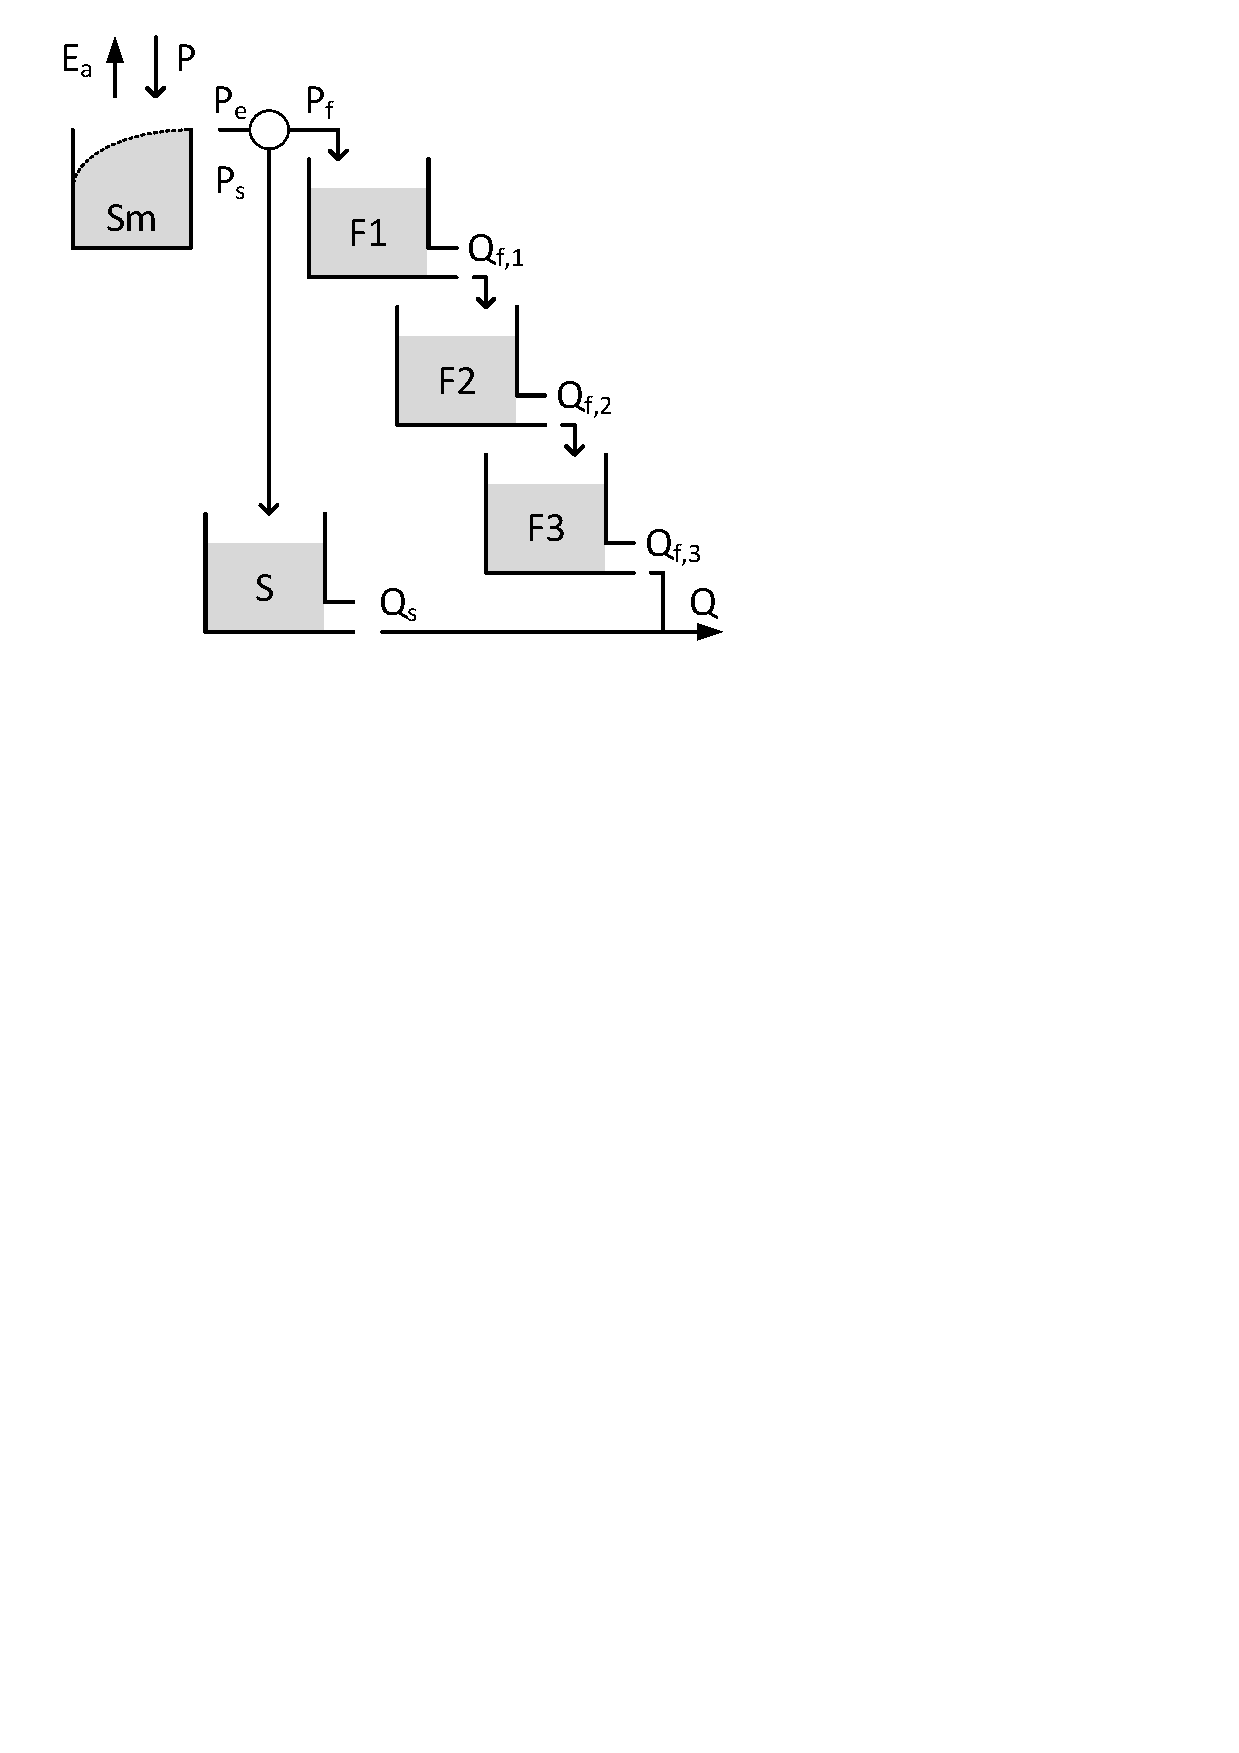
\includegraphics[trim=1cm 18.5cm 7cm 1cm,width=7cm,keepaspectratio]{./AppA_files/29_schematic.pdf}
\caption{Structure of the HyMOD model} \label{fig:29_schematic}
\end{wrapfigure}

\begin{align}
	\frac{dSm}{dt} &= P-E_a-P_e \\
	E_a &= \frac{Sm}{S_{max}}*E_p\\
	P_e &= \left(1-\left(1-\frac{S}{S_{max}}\right)^b\right)*P
\end{align}

Where Sm is the current storage in Sm [mm], $S_{max}$ [mm] is the maximum storage in Sm, $E_a$ and $E_p$ the actual and potential evapotranspiration respectively [mm/d] and b is the soil depth distribution parameter [-]. P [mm/d] is the precipitation input.

\begin{align}
	\frac{dF_1}{dt} &= P_f - Q_{f,1}\\
	P_f &= a*P_e \\
	Q_{f,1} &= k_f*S_{f,1} 
\end{align}

} % end of wrapfigure fix

\noindent Where $F_1$ is the current storage in store $F_1$ [mm], $a$ the fraction of $P_e$ that flows into the fast stores and $k_f$ the runoff coefficient of the fast stores. Stores $F_2$ and $F_3$ take the outflow of the previous store as input ($Q_{f,1}$ and $Q_{f,2}$ respectively) and generate outflow analogous to the equations above.

\begin{align}
	\frac{dS}{dt} &= P_s - Q_s\\
	P_s &= (1-a)*P_e \\
	Q_s &= k_s*S 
\end{align}
  
\noindent Where $S$ is the current storage in store S [mm], $1-a$ [-] the fraction of $P_e$ that flows into the slow store and $k_s$ the runoff coefficient of the slow store. Total outflow:

\begin{align}
	Q_t &= Q_s + Q_{f,3}
\end{align}

\subsection{Parameter overview}
% Table generated by Excel2LaTeX from sheet 'Sheet1'
\begin{table}[htbp]
  \centering
    \begin{tabular}{lll}
    \toprule
    Parameter & Unit  & Description \\
    \midrule
    $S_{max}$ & $mm$  & Maximum soil moisture storage \\
    $b$   & $-$   & Contributing area curve shape parameter \\
    $a$   & $-$   & Fraction of effective precipitation that is fast flow \\
    $k_f$ & $d^{-1}$ & Runoff coefficient \\
    $k_s$ & $d^{-1}$ & Runoff coefficient \\
    \bottomrule
    \end{tabular}%
  \label{tab:addlabel}%
\end{table}%
